% 12 pt, 1 inch margin, 1.5 line spacing
\documentclass[12pt, oneside]{article}
\usepackage{geometry}
\geometry{letterpaper, margin=1in}

\usepackage[utf8]{inputenc}
\usepackage[T1]{fontenc}
\usepackage[english]{babel}
\usepackage{graphicx}
\usepackage{amssymb}
\usepackage{authblk}
\usepackage{setspace}
\usepackage{tabularx}
\usepackage{hyperref}
\usepackage{adjustbox}
\usepackage{listings}
\usepackage{float}
\onehalfspacing


% changes Twitter to be specific
\title{Measuring and Forecasting Influenza \\
  Outbreaks Using Twitter \\
  \large Technical Report}

\author[1]{Tianyu Chen}
\author[2]{Yuhan Zeng}
\author[1]{Rui Zhang}
\affil[1]{Department of Computer Science, Indiana University}
\affil[2]{Department of Chemistry, Indiana University}
\affil[ ]{\textit{chen512@indiana.edu, \{rz20, yuhzeng\}@iu.edu}}
\renewcommand\Authands{, }
\date{\today}
\begin{document}
\maketitle




\section{Objectives and Significance}

% Briefly introduce the significance of the project. ** 1 ~ 3 paragraphs **

Infectious diseases are one of the major causes of morbidity and mortality, among which influenza is a ubiquitous epidemic \cite{hickmann2015forecasting}.
Commonly known as ``the flu'', it is caused by influenza virus and can be a highly infectious disease whose symptoms include runny nose, (high) fever,
sore throat, headache, coughing and fatigue\cite{wiki:flu}. Although there are numerous studies about predicting and forecasting the trend of influenza outbreaks,
there are some limitations still, specifically of their source of data. Related studies commonly leverage influenza-like illness (ILI) and severe acute
respiratory infections (SARI) data, which is defined by WHO\cite{world2014global}. Take the \textit{Influenza Observation and Forecast} system that is part of
Columbia Prediction of Infectious Disease (CPID) maintained by Columbia University \cite{cpid} for example, it only tracks the data from a total of 38 out of
195 sovereignties in the world today. Furthermore, its frequency of prediction can be limited by the publication of the corresponding data source.

To mitigate the problems above, we propose an epidemic outbreak prediction technique based on analyzing the data gathered from popular social media
like Twitter. Compared with the traditional approach, a noteworthy advantage of social media information is its ubiquitousness and timeliness
- end users are producing such data wherever and whenever they are. By performing a keyword-based text mining based on an anonymized tweet dataset and utilizing
the geographic information as a supplement, we can forecast whether a influenza outbreak is expected in near future.




\section{Background}

% 1. Introduce all important concepts and background information
% 2. Search the literature and describe previous work on this problem
% 3. If there exists previous work on the problem, describe what makes your work particularly interesting
% ** 1 ~ 2 pages **

\subsection{Predicting the Flu}

Influenza, often called ``the flu'', is an acute respiratory illness that infects approximately 10 - 15\% of the people around the world each year.
It can be deadly. For example in 2009, pandemic H1N1 (\textit{``swine flu''}) is estimated to result in 12,469 deaths in the United States \cite{H1N1}.
The early detection of influenza is of paramount importance to timely contain the spread of the illness. In the United States, Centers for Disease Control and Prevention (CDC)
report an influenza-like illness (ILI) index weekly based on the data collected from medical practices in a surveillance network. However, this report process is almost
entirely manual and there is a typical 1 - 2 week delay due to the lag in clinical data acquisition \cite{TwitterSeasonalFlu}.
Given the increasing demand for epidemic monitoring and forecasting in real time, web and social media (such as Google \cite{GoogleFlu} and Twitter \cite{TwitterFlu})
emerge as a new data source \cite{MediaFlu}.

\subsection{Twitter Text Mining}

Twitter, an online micro-blogging (limited to 280 characters) and social network service, has an average of 330 million active users worldwide \cite{TwitterUser} each month.
It could be a promising data source for the early detection of ILI due to its timeliness, public availability, and popularity \cite{TwitterAnalyzeMessage}.
Paul et al. \cite{TwitterWorldWide} shows that influenza-related tweets were positively correlated ($r$: 0.37 - 0.81) with existing government surveillance data
in 10 English-speaking countries.

\subsubsection{The Twitter API}
\label{subsubsec:api}

\begin{table}[h]
  \centering
  \caption{A list of Twitter APIs}
  \label{table:api}
  \begin{tabularx}{.75\textwidth}{ |c|c|X| }
    \hline
    \textbf{Parameter} & \textbf{Required} & \textbf{Function} \\
    \hline
    \hline
    q & Yes & The query string, 500 chars max \\
    \hline
    geocode & No & Specifying the latitude/longitude as well as the radius \\
    \hline
    lang & No & ISO 639-1 language code, restricting the results \\
    \hline
    locale & No & Specifying the language of the query string \\
    \hline
    result\_type & No & Has 3 values: \textit{recent} (only recent results), \textit{popular} (only popular ones) and \textit{mixed} (all tweets) \\
    \hline
    count & No & The number of tweets returned \\
    \hline
    until & No & Tweets created before a specific date \\
    \hline
  \end{tabularx}
\end{table}

% Briefly introduce a few useful APIs provided by Twitter
The Twitter API is an interface that takes a query as input and returns a JSON containing relative tweets and metadata as output.
In Table ~\ref{table:api} some parameters that we are interested in are listed with their functionalities.

\subsubsection{Online Twitter Archives}
\label{subsubsec:archives}

There are multiple online pre-grabbed archives of Twitter streams for general research purposes. In our experiment, we use the pre-grabbed online streams from Archive Team,
which are packed into tarballs and ready to download \footnote{\url{https://archive.org/details/twitterstream}}.

The dataset is in JSON format and the fields are as described in section ~\ref{subsubsec:api}. The data is annotated with date in the directory hierarchy. However,
the tweets contained in the dataset are worldwide without passsing through any filter. We perform data cleansing to ensure that the preprocessed dataset only
contains the tweets that we are interested in and the number of the tweets are large enough for a meaningful result and relatively small enough that it is still
within our processing ability.

The data cleansing and preprocessing techniques are explained in detail in section ~\ref{subsec:data_collection}.

\subsubsection{Related Research}

A variety of data mining and machine learning techniques have been applied to Twitter data analysis and influenza trend prediction.
Santillana et al. \cite{Santillana} combine multiple ILI activity estimates into a single prediction of ILI using machine learning ensemble approaches,
which produces accurate weekly ILI predictions for up to four weeks ahead of CDC's ILI reports. Santos et al. \cite{Santos} show that by changing data pre-processing and
feature extraction and selection the Naive-Bayes classifier and regression model built to predict the flu can be adapted to languages other than English.
Aron Culotta \cite{Culotta} proposes a document classifier to filter the \textit{misleading} messages, which significantly reduce error rate in simulated false alarm experiments.
Li et al. \cite{Li} build up a real-time ILI reporting system based on Flu Markov Network (Flu-MN), an unsupervised Bayesian algorithm based on a 4 phase Markov Network.
Chen et al. \cite{Chen} propose both an unsupervised model and an improved supervised weakly model that captures the hidden states of a user from her tweets
and estimates the flu trend. Aramaki et al. \cite{Aramaki} describe a support vector machine (SVM) based classifier that shows high correlation (0.97)
at the outbreak and early spread. Achrekar et al. \cite{TwitterSeasonalFlu} show that text mining significantly enhances the correlation between the Twitter and CDC reported ILI rates.

In particular, Lee et al. \cite{TwitterSurveillance} reports a real-time flu surveillance system leveraging data mining on tweets. However, their approach only accounts for
a few most \textit{frequent} words that co-occurs with a disease name, which seems na\"{i}ve in that the model overlooks \textit{infrequent} keywords related to flu outbreak.
They update their system in 2017 \cite{TwitterNNs} using multilayer perceptron. Compared to their previous work, it shows an improved accuracy.
However, only promoting tweets (ads) and the repeated ones are filtered.




\section{Methodology}
\label{sec:methodology}
% ** 2 ~ 4 pages! **

\subsection{Data Collection}
\label{subsec:data_collection}

% 1. Describe your data and how you will obtain it

Social media like Twitter and Facebook plays an important role in our daily life today. Organizations such as Centers for Disease Control and Prevention
(CDC) collect weekly influenza test results from public health laboratories and make infection prediction with an inevitable delay of up to two weeks.
For a more timely and efficient prediction of influenza, we collect a vast number of tweets that fall into a particular time span and extract related data
from them. Owing to the popularity and timeliness of Twitter posts, they can be used to assess health status or predict the spread and fluctuation of an epidemic
in a certain population in real-time.

\subsubsection{Data Collection and Preprocessing}

As is mentioned in ~\ref{subsubsec:archives}, we collect Twitter streams from the Archive Team online archive. Then we filter the tweets through a preprocessing
script that sorts out the tweets whose \path{location} field contains either the full name of one the states in the United States or the abbreviation.

We store the processed tweets in pickle \footnote{\url{https://docs.python.org/3/library/pickle.html}} binary object serialization format for further processing.
One tweet object is a dictionary that contains 4 fields - week, date, location and text. Week and date represent the time at which the tweet is generated. We care
about the week number since the CDC reports are organized in weeks. Location are extracted from the \path{location} field of the original tweet. Text contains the
plain text content of the tweet, on which further natural language processing is performed to determine whether it is flu related.

\begin{lstlisting}[caption={A sample preprocessed tweet}]
{'date': '2017-10-01',
 'location': 'LA (Lower Alabama)',
 'text': "RT @ClayTravis: Wow, Budweiser's getting so many calls
          demanding they drop NFL sponsorship that their official
          phone bank addresses it. Cal...",
 'week': 39}
\end{lstlisting}

We collect and process the tweets from October, 2017 to December, 2017 (12 weeks).
There are over 200,000 tweets every day that are identified to be located within the U.S.

\subsubsection{Manual Labelling}

We manually label a random portion of the dataset. The label represents whether the corresponding tweet is related to influenza (0 or 1) and serves as a groundtruth.

Since the portion of flu correlated tweets is small and it is time consuming to look at all of them, we first narrow down the scope using a set of heuristics.
The heuristics are a series of keywords that fall into 3 categrories - flu names, symptoms and treatments.

\begin{table}[h]
  \centering
  \caption{Heuristics keywords}
  \label{table:heuristics}
  \begin{tabularx}{.7\textwidth}{ |c|X| }
    \hline
    \textbf{Category} & \textbf{Keywords} \\
    \hline
    \hline
    Names & flu influenza h5n1 h1n1 \\
    \hline
    Symptoms & cough fever headache sore throat \newline sorethroat sneez vomit runny nose \newline runnynose fatigue \\
    \hline
    Treatments & tamiflu tylenol theraflu advil mucinex \newline benadry corenza \\
    \hline
  \end{tabularx}
\end{table}

The manually labelled data is used for keywords extraction.

\subsection{Implementation}

% 2. Describe your methodology: give flowcharts, diagrams, pseudocode or formulas where appropriate
% ** This section needs significant refactoring! **

\subsubsection{Keyword Extraction}

To provide a better insight of a Twitter based trend predictor and to reduce the data dimensionality, we text mine the keywords
from the datasets collected using a methodology described in ~\ref{subsec:data_collection}. We used  $\chi^2$-test, which assesses the independence
of each word against the relevance label. The rationale behind the test is that, suppose a word occurs in a probability $P(W)$
and a tweet is flu relevant in a probability of $P(R)$, if a word is flu irrelevant, then we expect the independence of joint probability
(i.e the probability of this word occurring in a informative tweet) to be $P(W, R) = P(W) \times P(R)$. The $\chi^2$ parameter is calculated by:

$$ \chi_c^2 = \sum{\frac{(O_i-E_i)^2}{E_i}}$$

where $c$ is the degree of freedom, $O_i$ is the observation and $E_i$ is the expected value.
An advantage of $\chi^2$-test is its fast performance compared to the Wilcoxon-rank test that appears in our proposal,
which requires exhaustively building random forests to estimate the significance of each word.
By setting up a $p-value$ threshold, we can skip the words that are not strongly associated with the relevance labels.

\subsubsection{Predictive Model}

We employ a neural network (NN) that involves a multilayer regressor to predict the flu trend.
We combine the ILI-related physician visit percentage with the term frequencies of the keywords in each tweet as input
and produce the influenza statistics in the following week as output.
It is worth mentioning that our approach introduces a keywords list to filter the tweets so that the dimensionality of dataset can be significantly reduced.
This is important to improve the efficiency of the predictor especially when we have such a big pool of tweets.
The training and testing samples are prepared by the preprocessing scripts.
The \path{sklearn.neural_network.MLPRegressor} from machine learning library \path{scikit-learn v0.19.1} is used to build the neural network.

\subsection{Evaluation Strategy}
\label{subsec:evaluation}

% 3. Describe evaluation strategy in detail

Aside from a direct comparison of flu activities between prediction and real statistics data,
we also measure the performance of the predictive model in 3 evaluation metrics including
Pearson correlation, mean squared error (MSE), and mean absolute error (MAS).

\paragraph{Pearson Correlation}
Pearson Correlation ($r$) is a measure of the linear correlation between two variables $X$ and $Y$ \cite{wiki:correlation}.

$$ r = \frac{\sum_{i=1}^n(x_i-\bar{x})(y_i-\bar{y})}{\sqrt{\sum_{i=1}^n(x_i-\bar{x})^2}\sqrt{\sum_{i=1}^n((y_i-\bar{y})^2}}$$

\paragraph{Mean Squared Error}
Mean Squared Error (MSE) is a measure of the difference between predicted and real values \cite{wiki:root-mean-square}.

$$MSE = \frac{\sum_{i=1}^{n}(\hat{y}-y_i)^2}{n}$$

\paragraph{Mean Absolute Error}
Mean Absolute Error (MAE) is also a measure of the difference between predicted and real values \cite{wiki:mean-absolute-error}, which takes absolute value instead of square.
It may be more desirable than MSE in certain circumstances such as easy interpretation and handling large errors \cite{wiki:mean-absolute-error-root-mean-square}.

$$MAE = \frac{\sum_{i=1}^{n}|\hat{y}-y_i)|}{n}$$

\section{Results}

% 1. Present here all your results and findings
% 2. Describe experiments done for each figure and table
% 3. Provide headers for all your tables and make sure it is easy to understand what your results are
% ** 5 ~ 6 pages! **

\subsection{A Small Dataset}
To develop a reliable method to extract the keywords for flu trend prediction, we first study the same datasets
used by Lamb et al. \cite{lamb-paul-dredze-naacl-2013}. The keywords automatically generated by our methods are evaluated manually,
to ensure a good coverage of relevant information while keep a small feature size.

\subsubsection{2012 Twitter Dataset}
Lamb et al. \cite{lamb-paul-dredze-naacl-2013} collect and manually label 4,760 tweets in the year of 2012 \cite{lamb-paul-dredze-naacl-2013}.
Due to Twitter guidelines, the authors only release the \textit{id}s of the tweets without attaching the original text contents.
Unfortunately, the Twitter APIs have a strict limitation of the tweets that one can obtain under a standard developer account.
\footnote{Twitter developer platform\url{https://developer.twitter.com/}} - only 20 tweets can be downloaded.
Considering such a restriction, we use the pre-grabbed twitter dataset mentioned in ~\ref{subsubsec:archives} for further studies.

\subsubsection{Keyword Extraction}
A few downloaded tweets are shown in Table \ref{table:sampler}. It is worth mentioning that all tweets shown contain the words ``flu''.
However, only a portion of the tweets are relevant to influenza outbreaks. For example, ``getting swine flu vaccine within 4 weeks'' is no more than an advertisement,
while ``@mmWine matty, you have the bird flu! Depends, what cha got going on?!? \& 1'' implies that the party concerned is potentially infected and is thus relevant.
The subtle difference between relevant and irrelevant content poses a challenge for a reliable prediction, especially using a bag-of-word model.


\begin{table}[h!]
\centering
\begin{adjustbox}{max width=\textwidth}
 \begin{tabular}{| l | c |} 
 \hline
 \textbf{Tweets} & \textbf{relevance} \\ [0.5ex]
 \hline
 \hline
 RT @EWJJr: Difference between bird flu \& swine flu: For bird flu you get tweetment. For swine flu you get oinkment. /That's so bad it's good & 0 \\
 Illinois getting swine flu vaccine within 4 weeks http://bit.ly/11chvS & 0\\
 RT @EWJJr: Difference between bird flu \& swine flu: For bird flu you get tweetment. For swine flu you get oinkment. /That's so bad it's good & 0 \\
 RT @WatchBirds Bird News: Missoula waterfowl tested for bird flu http://bit.ly/17V9or  & 0 \\
 i know it's not "swine flu"! no urge to to poop in the mud and roll around in it. NOT "bird flu"- no poopin' on windshields or statues. & 0\\
 Swine Flu - How worried are you? - Take our poll now and check out how others feel! http://bit.ly/A07Zq - Vote Today! & 1\\
 @killerbarbiex3 nah u good... if u did i wouldnt reply to u lol, I cant afford to get the Bird Flu! lol & 1\\
 Even @BarackObama got the Twitter Bird Flu!! & 0\\
 @TiernanDouieb It's bird flu mate - it's mutated with twitter.& 0 \\
 HA @ twitter catching the bird flu & 0\\
 Ohhhh... I got Twitter bird flu too... I match @teresakopec & 0\\
 @AMAZINGBOSSUP bird flu goin around on twitter & 0\\
 RT @jryanlaw: Ohhhh... I got Twitter bird flu too... I match @teresakopec //Did you sneeze on your hand or your elbow young lady??? & 0 \\
 bird flu! & 0 \\
 RTxoxonosheenRT @laurawalker86 my twitter account has bird flu LOL ***lol I've recovered***---and mine is a pretty colour :) & 0\\
 @mmWine matty, you have the bird flu! Depends, what cha got going on?!? & 1 \\
 The approach of winter and flu has you worried? Worry no more Click Me for Health Now http://bit.ly/Tl8iC & 1\\
 RT @wickedpoptart: ooooooh nooooo lolRT @knaught09: @wickedpoptart @bluegrasspundit A case of bird flu? & 0\\
 @Star\_Qualities? AHHHHH you have bird flu.... Flap your wings so you can fly high & 0\\
 Realizing how stoked I really am to go to Norway on the 18th. Really stoked. do they still have bird flu over there? & 1\\
 \hline
 \end{tabular}
 \end{adjustbox}
 \caption{A Twitter content sampler (2012)}
\label{table:sampler}
\end{table}


We generate a list of keywords by $\chi^2$-test based on various statistics thresholds ($p-value$), as is shown in Table \ref{table:2}.
This keywords list does not even include ``flu'', which is due to the fact that all tweets contain the keyword of ``flu''.
We conclude that by using a small $p-value$ such as 0.01, it simple eliminates too many candidates.
While using a larger p-value such as 1.0 we can generate a large number of candidates, some words that do not make sense such as ``cha'' and ``u''
are also included in the result, which can be a potential issue especially in large datasets when we attempt to use small subsets of the words
in order to effectively decrease the dimensionality of the dataset. As a result, we decide to use $p-value=0.05$ to balance the number and the relevance.


\begin{table}[h!]
  \centering
  \begin{adjustbox}{max width=\textwidth}
    \begin{tabular}{|c|l|} 
      \hline
      \textbf{p-value} & \textbf{Keywords} \\ [0.5ex] 
      \hline
      \hline
      0.01 & [] \\
      0.05 & [worried] \\
      0.1 & [afford, approach, cha, check, click, depend, feel, health,\\ 
        & poll, realize, reply, stoke, today, u, vote, winter, worried, worry]\\
      \hline
    \end{tabular}
  \end{adjustbox}
  \caption{Keywords for the 2012 Twitter dataset}
  \label{table:2}
\end{table}


\subsection{Flu Trend Prediction on the Small Dataset}
After implementing the keyword extraction algorithm as a way of feature selection, we propose to employ neural network (NN) with regression  
to predict the flu trend. The groundtruth of flu activities in the United States is obtained from CDC report on the percentage weighted influenza-like illness
(\%-weighted ILI). We intend to predict the flu trend (whether the number of patients increases or decreases) as well as the \%-weighted ILI.

\subsubsection{2015-2016 Twitter Dataset}
The two datasets are obtained from online resources in a blog post \cite{small-datasets}, which contain a random sample of 1,000 tweets
collected between September 2015 to April 2016. Each tweet in those datasets were also labelled as either ``relevant'' or ``irrelevant'',
according to the fact whether the one who posts the tweet need a flu shot or not \cite{small-datasets}.
This datasets could be a good starting point to develop our framework, since all the tweets had been labeled and the overall datasets size is relatively small. 

\subsubsection{Keyword Extraction}
We also extract a list of keywords on the 2015-2016 Twitter dataset using the previously described method, as is shown in Table \ref{table:3}.
Herein, the keywords are classified into groups according to their meaning and implication.
It is worth mentioning that our method is able to capture the relevant words such as those in ``medical'' and ``flu'' groups.

\begin{table}[h!]
  \centering
  \begin{adjustbox}{max width=\textwidth}
    \begin{tabular}{| l | l |} 
      \hline
      \textbf{Class} & \textbf{Keywords} \\ [0.5ex] 
      \hline
      \hline
      adv. & barely, probably, exactly, literally \\
      emotion & bitch, stupid, brave, ouch, wow \\
      flu names & bird, cold, hurt, influenza, sick, sore, swine \\
      glossaries & appointment, doctor, health, blood,  \\
      & needle, physical,  stomach, symptom, shot, virus \\
      time & ago mid, minute, morning, season, time, today, tomorrow, yesterday  \\
      verb. & catch, cry, deserve, feel, guess, hate, help, hit, know, like, pass, pump, stay \\
      noun. & arm, bed, case, clock, hop, job, news, outbreak, people, place, luck, man, shoulder, work  \\
      other & en, contra, de, la, plus, right, u \\
      \hline
    \end{tabular}
  \end{adjustbox}
  \caption{Keywords for the 2015-2016 Twitter datasets}
  \label{table:3}
\end{table}

We process the tweets using the bag-of-words (BoW) model into a numerical vector space and sum the term frequency (TF) of each keyword in every week.
The keyword extraction not only decreases the dimensionality of the dataset, but also improves the quality of the features. 
Such a conclusion is drawn from the most frequent words before and after keyword extraction, which are shown in Figure \ref{fig:1}.

\begin{figure}[h]
    \centering
    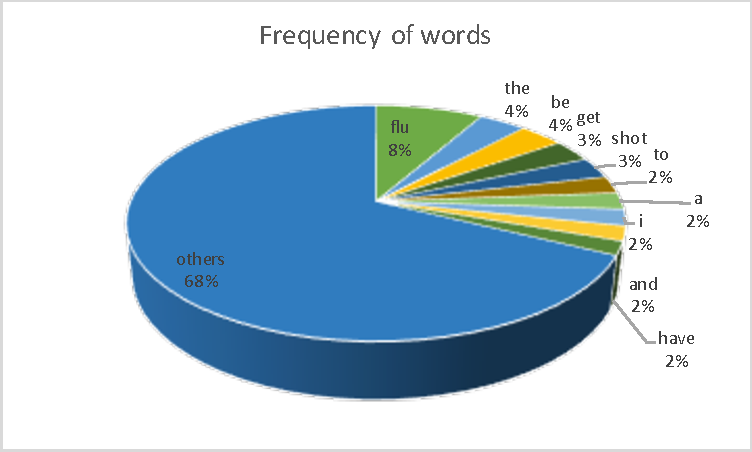
\includegraphics[width=0.7\textwidth]{fig1b}
    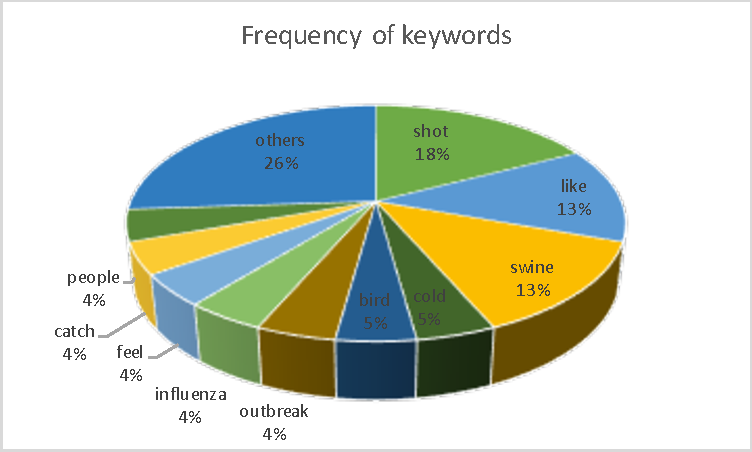
\includegraphics[width=0.7\textwidth]{fig1a}
    \caption{The term frequency in the 2015-2016 Twitter datasets. }
    \label{fig:1}
\end{figure}

\subsubsection{Trend Prediction}

We employ a multi-layer regressor to predict the percentage of weighted influenza-like illness (\%-weighted ILI, $y$) of all patients.
To improve the prediction accuracy, the input ($X$) contains not only the tweet vectors (from bag-of-words model and keyword extraction),
but also the \%-weighted ILI in the \textit{previous} week, which serves as a way to assess the historical influence and as a starting point
for flu trend prediction. It is also worth mentioning that we can actually use the \%-weighted ILI from anytime in the past, for example, the last three weeks
or even add some noise to the factor, like a small random perturbation on the percentage, which better simulates the reality.

\begin{figure}[h]
  \centering
  \scalebox{0.85}{% GNUPLOT: LaTeX picture with Postscript
\begingroup
  \makeatletter
  \providecommand\color[2][]{%
    \GenericError{(gnuplot) \space\space\space\@spaces}{%
      Package color not loaded in conjunction with
      terminal option `colourtext'%
    }{See the gnuplot documentation for explanation.%
    }{Either use 'blacktext' in gnuplot or load the package
      color.sty in LaTeX.}%
    \renewcommand\color[2][]{}%
  }%
  \providecommand\includegraphics[2][]{%
    \GenericError{(gnuplot) \space\space\space\@spaces}{%
      Package graphicx or graphics not loaded%
    }{See the gnuplot documentation for explanation.%
    }{The gnuplot epslatex terminal needs graphicx.sty or graphics.sty.}%
    \renewcommand\includegraphics[2][]{}%
  }%
  \providecommand\rotatebox[2]{#2}%
  \@ifundefined{ifGPcolor}{%
    \newif\ifGPcolor
    \GPcolortrue
  }{}%
  \@ifundefined{ifGPblacktext}{%
    \newif\ifGPblacktext
    \GPblacktexttrue
  }{}%
  % define a \g@addto@macro without @ in the name:
  \let\gplgaddtomacro\g@addto@macro
  % define empty templates for all commands taking text:
  \gdef\gplbacktext{}%
  \gdef\gplfronttext{}%
  \makeatother
  \ifGPblacktext
    % no textcolor at all
    \def\colorrgb#1{}%
    \def\colorgray#1{}%
  \else
    % gray or color?
    \ifGPcolor
      \def\colorrgb#1{\color[rgb]{#1}}%
      \def\colorgray#1{\color[gray]{#1}}%
      \expandafter\def\csname LTw\endcsname{\color{white}}%
      \expandafter\def\csname LTb\endcsname{\color{black}}%
      \expandafter\def\csname LTa\endcsname{\color{black}}%
      \expandafter\def\csname LT0\endcsname{\color[rgb]{1,0,0}}%
      \expandafter\def\csname LT1\endcsname{\color[rgb]{0,1,0}}%
      \expandafter\def\csname LT2\endcsname{\color[rgb]{0,0,1}}%
      \expandafter\def\csname LT3\endcsname{\color[rgb]{1,0,1}}%
      \expandafter\def\csname LT4\endcsname{\color[rgb]{0,1,1}}%
      \expandafter\def\csname LT5\endcsname{\color[rgb]{1,1,0}}%
      \expandafter\def\csname LT6\endcsname{\color[rgb]{0,0,0}}%
      \expandafter\def\csname LT7\endcsname{\color[rgb]{1,0.3,0}}%
      \expandafter\def\csname LT8\endcsname{\color[rgb]{0.5,0.5,0.5}}%
    \else
      % gray
      \def\colorrgb#1{\color{black}}%
      \def\colorgray#1{\color[gray]{#1}}%
      \expandafter\def\csname LTw\endcsname{\color{white}}%
      \expandafter\def\csname LTb\endcsname{\color{black}}%
      \expandafter\def\csname LTa\endcsname{\color{black}}%
      \expandafter\def\csname LT0\endcsname{\color{black}}%
      \expandafter\def\csname LT1\endcsname{\color{black}}%
      \expandafter\def\csname LT2\endcsname{\color{black}}%
      \expandafter\def\csname LT3\endcsname{\color{black}}%
      \expandafter\def\csname LT4\endcsname{\color{black}}%
      \expandafter\def\csname LT5\endcsname{\color{black}}%
      \expandafter\def\csname LT6\endcsname{\color{black}}%
      \expandafter\def\csname LT7\endcsname{\color{black}}%
      \expandafter\def\csname LT8\endcsname{\color{black}}%
    \fi
  \fi
    \setlength{\unitlength}{0.0500bp}%
    \ifx\gptboxheight\undefined%
      \newlength{\gptboxheight}%
      \newlength{\gptboxwidth}%
      \newsavebox{\gptboxtext}%
    \fi%
    \setlength{\fboxrule}{0.5pt}%
    \setlength{\fboxsep}{1pt}%
\begin{picture}(7200.00,5040.00)%
    \gplgaddtomacro\gplbacktext{%
      \csname LTb\endcsname%%
      \put(814,767){\makebox(0,0)[r]{\strut{}$1$}}%
      \put(814,1346){\makebox(0,0)[r]{\strut{}$1.2$}}%
      \put(814,1925){\makebox(0,0)[r]{\strut{}$1.4$}}%
      \put(814,2504){\makebox(0,0)[r]{\strut{}$1.6$}}%
      \put(814,3082){\makebox(0,0)[r]{\strut{}$1.8$}}%
      \put(814,3661){\makebox(0,0)[r]{\strut{}$2$}}%
      \put(814,4240){\makebox(0,0)[r]{\strut{}$2.2$}}%
      \put(814,4819){\makebox(0,0)[r]{\strut{}$2.4$}}%
      \put(1009,484){\makebox(0,0){\strut{}2015}}%
      \put(1371,484){\makebox(0,0){\strut{}41}}%
      \put(1733,484){\makebox(0,0){\strut{}42}}%
      \put(2095,484){\makebox(0,0){\strut{}43}}%
      \put(2458,484){\makebox(0,0){\strut{}44}}%
      \put(3182,484){\makebox(0,0){\strut{}46}}%
      \put(3544,484){\makebox(0,0){\strut{}47}}%
      \put(4992,484){\makebox(0,0){\strut{}51}}%
      \put(6441,484){\makebox(0,0){\strut{}2016}}%
      \put(6803,484){\makebox(0,0){\strut{} 4}}%
    }%
    \gplgaddtomacro\gplfronttext{%
      \csname LTb\endcsname%%
      \put(330,2793){\rotatebox{-270}{\makebox(0,0){\strut{}percentage of weighted ILL}}}%
      \put(3906,154){\makebox(0,0){\strut{}time (weeks)}}%
      \csname LTb\endcsname%%
      \put(5816,4646){\makebox(0,0)[r]{\strut{}real}}%
      \csname LTb\endcsname%%
      \put(5816,4426){\makebox(0,0)[r]{\strut{}predict}}%
    }%
    \gplbacktext
    \put(0,0){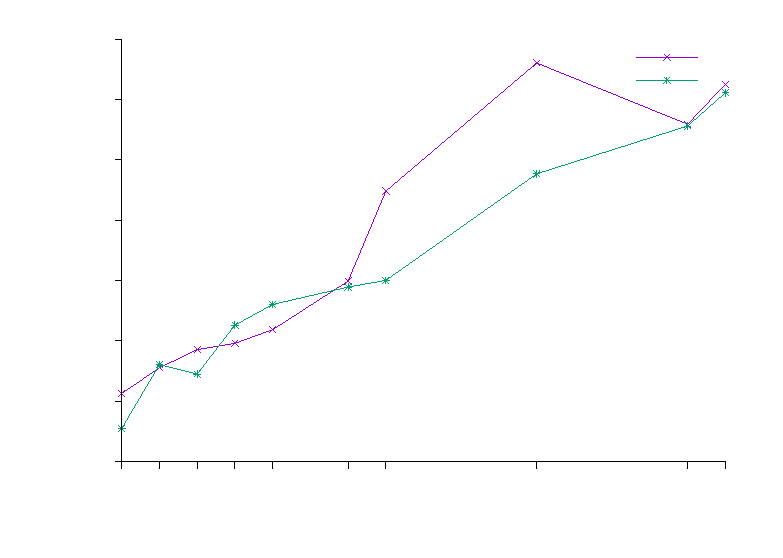
\includegraphics{plot_2}}%
    \gplfronttext
  \end{picture}%
\endgroup
}
  \caption{2015-2016 flu trend timeline}
  \label{figure:2}
\end{figure}

To evaluate the effectiveness of neural network on prediction, we processe the dataset per week as is described in the methodology section ~\ref{sec:methodology},
and randomly pick 50\% of the weeks for training while hold the remaining weeks for testing (1:1). After parameter optimization, we chose to set \path{lbfgs},
a quasi-Newton method, for weight optimization. We use the logistic sigmoid as the activation function and add two hidden layers (200 and 100 hidden units respectively)
\cite{nn-mlpregressor}. The predicted trend and the groundtruth are both shown in Figure ~\ref{figure:2}.


\subsection{Flu Trend Prediction on a Larger Dataset}

To evaluate our method on real world data, we make use of a relatively large dataset that contains millions of tweets.
We randomly sample a small portion of the tweets for manual labelling based on whether the content is relevant to flu outbreaks or not.
Keywords are subsequently generated by $\chi^2$-test.
The whole dataset is then processed with the keywords list as is described in the methodology section ~\ref{sec:methodology}.
We use the previously mentioned neural network (NN) developed for flu trend prediction and compare the predicted results with the ones on the CDC report,
which serve as groundtruth for our study.

\subsubsection{2017 Twitter Dataset (Large)}
The dataset used in this section is obtained from the Archive Team Twitter stream \cite{tweets-archive} ~\ref{subsec:data_collection},
which is a randomly collected JSON format dataset from general Twitter stream.
The original dataset is extremely large (over 1 GB tarball for a single day) and simply impractical to used them as a whole.
We cherrypick 3 months - October, November, and December in 2017.
There are 7,001,557 recorded tweets in October, 5,198,021 in November, and 6,739,178 in December, which are huge numbers.
To simplify the computing task, we perform the flu trend prediction on each month seperately.
We further randomly divide each month's tweets into 20 equally sized \textit{chunks},
which multiplex the number of training samples. After keyword extraction we get 279 keywords generated from 5,346 manually labeled tweets in October, 247 keywords from 4,276 tweets in October, and 404 keywords from 6,368 tweets in December respectively.

\subsubsection{Trend Prediction}


\begin{table}[H]
  \centering
  \begin{adjustbox}{max width=\textwidth}
    \begin{tabular}{| c | c | c | c | c |} 
      \hline
      \textbf{Month} & \textbf{k-fold} & \textbf{MSE} & \textbf{MAE} & \textbf{$R^2$} \\ [0.5ex] 
      \hline
      \hline
      Oct. & 1& 0.0017 & 0.0328 & 0.9518 \\
      & 2 & 0.0008 & 0.0210 & 0.9797 \\
      & 3 & 0.0007 &  0.0217 & 0.9814 \\
      & 4 & 0.0006 & 0.0187 & 0.9843 \\
      & 5 & 0.0084 & 0.0504 & 0.7792 \\
      Nov. & 1& 0.0007 & 0.0228 & 0.9858 \\
      & 2 & 0.0007 & 0.0210 & 0.9891 \\
      & 3 & 0.0009 &  0.0275 & 0.9794 \\
      & 4 & 0.0007 & 0.0228 & 0.9876 \\
      & 5 & 0.0035 & 0.0300 & 0.9244 \\
      Dec. & 1& 0.0166 & 0.1014 & 0.921 \\
      & 2 & 0.0068 & 0.0663 & 0.9976 \\
      & 3 & 0.0068 & 0.0691 & 0.9959 \\
      & 4 & 0.0144 & 0.0995 & 0.9927 \\
      & 5 & 0.7834 & 0.3818 & 0.6080 \\
      \hline
    \end{tabular}
  \end{adjustbox}
  \caption{The performance of neural network prediction}
  \label{table:4}
\end{table}


Leveraging the multilayer regressor, we get a flu trend timeline prediction as is shown in Figure \ref{figure:3},
\ref{figure:4} and \ref{figure:5} by a 66:33 split on the original dataset.
We also conduct a measurement on the mean squared error (MSE), mean absolute error (MAE), and Pearson correlation (corr) by a 5-fold cross-validation,
as is shown in Table \ref{table:4}.
It is apparent that our predictor generally performs well except for the last week of December, which is consistent with our cross-validation results (Table \ref{table:4}).
It also shows a high $R^2$ around 0.9 and a low MSE/MAE $< 0.1$, which suggests a promising application of our keyword extraction and neural network prediction model
in a general real-world flu trend prediction problem.

\begin{figure}[H]
  \centering
  \scalebox{0.85}{% GNUPLOT: LaTeX picture with Postscript
\begingroup
  \makeatletter
  \providecommand\color[2][]{%
    \GenericError{(gnuplot) \space\space\space\@spaces}{%
      Package color not loaded in conjunction with
      terminal option `colourtext'%
    }{See the gnuplot documentation for explanation.%
    }{Either use 'blacktext' in gnuplot or load the package
      color.sty in LaTeX.}%
    \renewcommand\color[2][]{}%
  }%
  \providecommand\includegraphics[2][]{%
    \GenericError{(gnuplot) \space\space\space\@spaces}{%
      Package graphicx or graphics not loaded%
    }{See the gnuplot documentation for explanation.%
    }{The gnuplot epslatex terminal needs graphicx.sty or graphics.sty.}%
    \renewcommand\includegraphics[2][]{}%
  }%
  \providecommand\rotatebox[2]{#2}%
  \@ifundefined{ifGPcolor}{%
    \newif\ifGPcolor
    \GPcolortrue
  }{}%
  \@ifundefined{ifGPblacktext}{%
    \newif\ifGPblacktext
    \GPblacktexttrue
  }{}%
  % define a \g@addto@macro without @ in the name:
  \let\gplgaddtomacro\g@addto@macro
  % define empty templates for all commands taking text:
  \gdef\gplbacktext{}%
  \gdef\gplfronttext{}%
  \makeatother
  \ifGPblacktext
    % no textcolor at all
    \def\colorrgb#1{}%
    \def\colorgray#1{}%
  \else
    % gray or color?
    \ifGPcolor
      \def\colorrgb#1{\color[rgb]{#1}}%
      \def\colorgray#1{\color[gray]{#1}}%
      \expandafter\def\csname LTw\endcsname{\color{white}}%
      \expandafter\def\csname LTb\endcsname{\color{black}}%
      \expandafter\def\csname LTa\endcsname{\color{black}}%
      \expandafter\def\csname LT0\endcsname{\color[rgb]{1,0,0}}%
      \expandafter\def\csname LT1\endcsname{\color[rgb]{0,1,0}}%
      \expandafter\def\csname LT2\endcsname{\color[rgb]{0,0,1}}%
      \expandafter\def\csname LT3\endcsname{\color[rgb]{1,0,1}}%
      \expandafter\def\csname LT4\endcsname{\color[rgb]{0,1,1}}%
      \expandafter\def\csname LT5\endcsname{\color[rgb]{1,1,0}}%
      \expandafter\def\csname LT6\endcsname{\color[rgb]{0,0,0}}%
      \expandafter\def\csname LT7\endcsname{\color[rgb]{1,0.3,0}}%
      \expandafter\def\csname LT8\endcsname{\color[rgb]{0.5,0.5,0.5}}%
    \else
      % gray
      \def\colorrgb#1{\color{black}}%
      \def\colorgray#1{\color[gray]{#1}}%
      \expandafter\def\csname LTw\endcsname{\color{white}}%
      \expandafter\def\csname LTb\endcsname{\color{black}}%
      \expandafter\def\csname LTa\endcsname{\color{black}}%
      \expandafter\def\csname LT0\endcsname{\color{black}}%
      \expandafter\def\csname LT1\endcsname{\color{black}}%
      \expandafter\def\csname LT2\endcsname{\color{black}}%
      \expandafter\def\csname LT3\endcsname{\color{black}}%
      \expandafter\def\csname LT4\endcsname{\color{black}}%
      \expandafter\def\csname LT5\endcsname{\color{black}}%
      \expandafter\def\csname LT6\endcsname{\color{black}}%
      \expandafter\def\csname LT7\endcsname{\color{black}}%
      \expandafter\def\csname LT8\endcsname{\color{black}}%
    \fi
  \fi
    \setlength{\unitlength}{0.0500bp}%
    \ifx\gptboxheight\undefined%
      \newlength{\gptboxheight}%
      \newlength{\gptboxwidth}%
      \newsavebox{\gptboxtext}%
    \fi%
    \setlength{\fboxrule}{0.5pt}%
    \setlength{\fboxsep}{1pt}%
\begin{picture}(7200.00,5040.00)%
    \gplgaddtomacro\gplbacktext{%
      \csname LTb\endcsname%%
      \put(814,767){\makebox(0,0)[r]{\strut{}$1.1$}}%
      \put(814,1274){\makebox(0,0)[r]{\strut{}$1.2$}}%
      \put(814,1780){\makebox(0,0)[r]{\strut{}$1.3$}}%
      \put(814,2287){\makebox(0,0)[r]{\strut{}$1.4$}}%
      \put(814,2793){\makebox(0,0)[r]{\strut{}$1.5$}}%
      \put(814,3300){\makebox(0,0)[r]{\strut{}$1.6$}}%
      \put(814,3806){\makebox(0,0)[r]{\strut{}$1.7$}}%
      \put(814,4313){\makebox(0,0)[r]{\strut{}$1.8$}}%
      \put(814,4819){\makebox(0,0)[r]{\strut{}$1.9$}}%
      \put(1009,484){\makebox(0,0){\strut{}$39$}}%
      \put(2168,484){\makebox(0,0){\strut{}$40$}}%
      \put(3327,484){\makebox(0,0){\strut{}$41$}}%
      \put(4485,484){\makebox(0,0){\strut{}$42$}}%
      \put(5644,484){\makebox(0,0){\strut{}$43$}}%
      \put(6803,484){\makebox(0,0){\strut{}$44$}}%
    }%
    \gplgaddtomacro\gplfronttext{%
      \csname LTb\endcsname%%
      \put(330,2793){\rotatebox{-270}{\makebox(0,0){\strut{}percentage of weighted ILL}}}%
      \put(3906,154){\makebox(0,0){\strut{}time (weeks)}}%
      \csname LTb\endcsname%%
      \put(5816,4646){\makebox(0,0)[r]{\strut{}real}}%
      \csname LTb\endcsname%%
      \put(5816,4426){\makebox(0,0)[r]{\strut{}predict}}%
    }%
    \gplbacktext
    \put(0,0){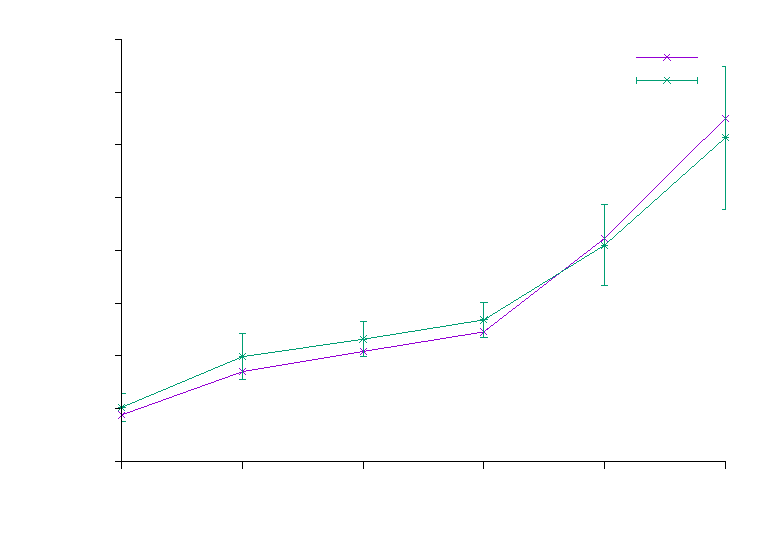
\includegraphics{plot_3}}%
    \gplfronttext
  \end{picture}%
\endgroup
}
  \caption{The flu trend timeline of Oct. 2017}
  \label{figure:3}
\end{figure}

\begin{figure}[H]
  \centering
  \scalebox{0.85}{% GNUPLOT: LaTeX picture with Postscript
\begingroup
  \makeatletter
  \providecommand\color[2][]{%
    \GenericError{(gnuplot) \space\space\space\@spaces}{%
      Package color not loaded in conjunction with
      terminal option `colourtext'%
    }{See the gnuplot documentation for explanation.%
    }{Either use 'blacktext' in gnuplot or load the package
      color.sty in LaTeX.}%
    \renewcommand\color[2][]{}%
  }%
  \providecommand\includegraphics[2][]{%
    \GenericError{(gnuplot) \space\space\space\@spaces}{%
      Package graphicx or graphics not loaded%
    }{See the gnuplot documentation for explanation.%
    }{The gnuplot epslatex terminal needs graphicx.sty or graphics.sty.}%
    \renewcommand\includegraphics[2][]{}%
  }%
  \providecommand\rotatebox[2]{#2}%
  \@ifundefined{ifGPcolor}{%
    \newif\ifGPcolor
    \GPcolortrue
  }{}%
  \@ifundefined{ifGPblacktext}{%
    \newif\ifGPblacktext
    \GPblacktexttrue
  }{}%
  % define a \g@addto@macro without @ in the name:
  \let\gplgaddtomacro\g@addto@macro
  % define empty templates for all commands taking text:
  \gdef\gplbacktext{}%
  \gdef\gplfronttext{}%
  \makeatother
  \ifGPblacktext
    % no textcolor at all
    \def\colorrgb#1{}%
    \def\colorgray#1{}%
  \else
    % gray or color?
    \ifGPcolor
      \def\colorrgb#1{\color[rgb]{#1}}%
      \def\colorgray#1{\color[gray]{#1}}%
      \expandafter\def\csname LTw\endcsname{\color{white}}%
      \expandafter\def\csname LTb\endcsname{\color{black}}%
      \expandafter\def\csname LTa\endcsname{\color{black}}%
      \expandafter\def\csname LT0\endcsname{\color[rgb]{1,0,0}}%
      \expandafter\def\csname LT1\endcsname{\color[rgb]{0,1,0}}%
      \expandafter\def\csname LT2\endcsname{\color[rgb]{0,0,1}}%
      \expandafter\def\csname LT3\endcsname{\color[rgb]{1,0,1}}%
      \expandafter\def\csname LT4\endcsname{\color[rgb]{0,1,1}}%
      \expandafter\def\csname LT5\endcsname{\color[rgb]{1,1,0}}%
      \expandafter\def\csname LT6\endcsname{\color[rgb]{0,0,0}}%
      \expandafter\def\csname LT7\endcsname{\color[rgb]{1,0.3,0}}%
      \expandafter\def\csname LT8\endcsname{\color[rgb]{0.5,0.5,0.5}}%
    \else
      % gray
      \def\colorrgb#1{\color{black}}%
      \def\colorgray#1{\color[gray]{#1}}%
      \expandafter\def\csname LTw\endcsname{\color{white}}%
      \expandafter\def\csname LTb\endcsname{\color{black}}%
      \expandafter\def\csname LTa\endcsname{\color{black}}%
      \expandafter\def\csname LT0\endcsname{\color{black}}%
      \expandafter\def\csname LT1\endcsname{\color{black}}%
      \expandafter\def\csname LT2\endcsname{\color{black}}%
      \expandafter\def\csname LT3\endcsname{\color{black}}%
      \expandafter\def\csname LT4\endcsname{\color{black}}%
      \expandafter\def\csname LT5\endcsname{\color{black}}%
      \expandafter\def\csname LT6\endcsname{\color{black}}%
      \expandafter\def\csname LT7\endcsname{\color{black}}%
      \expandafter\def\csname LT8\endcsname{\color{black}}%
    \fi
  \fi
    \setlength{\unitlength}{0.0500bp}%
    \ifx\gptboxheight\undefined%
      \newlength{\gptboxheight}%
      \newlength{\gptboxwidth}%
      \newsavebox{\gptboxtext}%
    \fi%
    \setlength{\fboxrule}{0.5pt}%
    \setlength{\fboxsep}{1pt}%
\begin{picture}(7200.00,5040.00)%
    \gplgaddtomacro\gplbacktext{%
      \csname LTb\endcsname%%
      \put(814,767){\makebox(0,0)[r]{\strut{}$1.7$}}%
      \put(814,1442){\makebox(0,0)[r]{\strut{}$1.8$}}%
      \put(814,2118){\makebox(0,0)[r]{\strut{}$1.9$}}%
      \put(814,2793){\makebox(0,0)[r]{\strut{}$2$}}%
      \put(814,3468){\makebox(0,0)[r]{\strut{}$2.1$}}%
      \put(814,4144){\makebox(0,0)[r]{\strut{}$2.2$}}%
      \put(814,4819){\makebox(0,0)[r]{\strut{}$2.3$}}%
      \put(1009,484){\makebox(0,0){\strut{}44}}%
      \put(2458,484){\makebox(0,0){\strut{}45}}%
      \put(3906,484){\makebox(0,0){\strut{}46}}%
      \put(5355,484){\makebox(0,0){\strut{}47}}%
      \put(6803,484){\makebox(0,0){\strut{}48}}%
    }%
    \gplgaddtomacro\gplfronttext{%
      \csname LTb\endcsname%%
      \put(330,2793){\rotatebox{-270}{\makebox(0,0){\strut{}percentage of weighted ILL}}}%
      \put(3906,154){\makebox(0,0){\strut{}time (weeks)}}%
      \csname LTb\endcsname%%
      \put(5816,1160){\makebox(0,0)[r]{\strut{}real}}%
      \csname LTb\endcsname%%
      \put(5816,940){\makebox(0,0)[r]{\strut{}predict}}%
    }%
    \gplbacktext
    \put(0,0){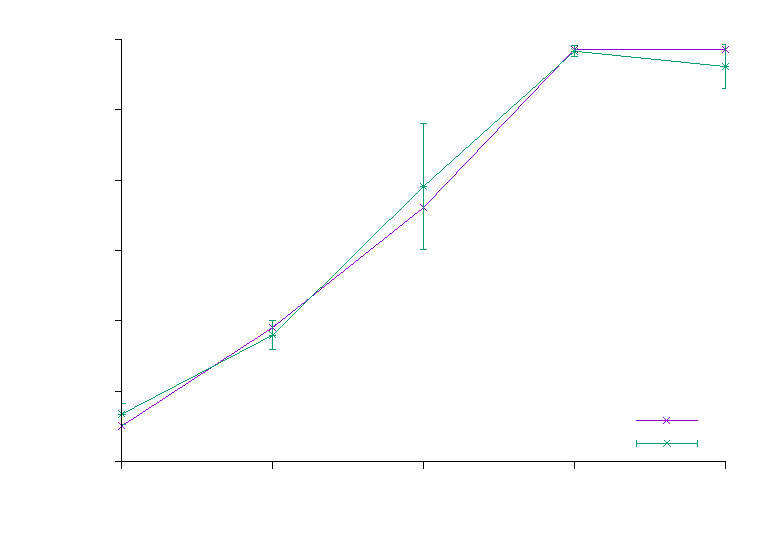
\includegraphics{plot_4}}%
    \gplfronttext
  \end{picture}%
\endgroup
}
  \caption{The flu trend timeline of Nov. 2017}
  \label{figure:4}
\end{figure}

\begin{figure}[H]
  \centering
  \scalebox{0.85}{% GNUPLOT: LaTeX picture with Postscript
\begingroup
  \makeatletter
  \providecommand\color[2][]{%
    \GenericError{(gnuplot) \space\space\space\@spaces}{%
      Package color not loaded in conjunction with
      terminal option `colourtext'%
    }{See the gnuplot documentation for explanation.%
    }{Either use 'blacktext' in gnuplot or load the package
      color.sty in LaTeX.}%
    \renewcommand\color[2][]{}%
  }%
  \providecommand\includegraphics[2][]{%
    \GenericError{(gnuplot) \space\space\space\@spaces}{%
      Package graphicx or graphics not loaded%
    }{See the gnuplot documentation for explanation.%
    }{The gnuplot epslatex terminal needs graphicx.sty or graphics.sty.}%
    \renewcommand\includegraphics[2][]{}%
  }%
  \providecommand\rotatebox[2]{#2}%
  \@ifundefined{ifGPcolor}{%
    \newif\ifGPcolor
    \GPcolortrue
  }{}%
  \@ifundefined{ifGPblacktext}{%
    \newif\ifGPblacktext
    \GPblacktexttrue
  }{}%
  % define a \g@addto@macro without @ in the name:
  \let\gplgaddtomacro\g@addto@macro
  % define empty templates for all commands taking text:
  \gdef\gplbacktext{}%
  \gdef\gplfronttext{}%
  \makeatother
  \ifGPblacktext
    % no textcolor at all
    \def\colorrgb#1{}%
    \def\colorgray#1{}%
  \else
    % gray or color?
    \ifGPcolor
      \def\colorrgb#1{\color[rgb]{#1}}%
      \def\colorgray#1{\color[gray]{#1}}%
      \expandafter\def\csname LTw\endcsname{\color{white}}%
      \expandafter\def\csname LTb\endcsname{\color{black}}%
      \expandafter\def\csname LTa\endcsname{\color{black}}%
      \expandafter\def\csname LT0\endcsname{\color[rgb]{1,0,0}}%
      \expandafter\def\csname LT1\endcsname{\color[rgb]{0,1,0}}%
      \expandafter\def\csname LT2\endcsname{\color[rgb]{0,0,1}}%
      \expandafter\def\csname LT3\endcsname{\color[rgb]{1,0,1}}%
      \expandafter\def\csname LT4\endcsname{\color[rgb]{0,1,1}}%
      \expandafter\def\csname LT5\endcsname{\color[rgb]{1,1,0}}%
      \expandafter\def\csname LT6\endcsname{\color[rgb]{0,0,0}}%
      \expandafter\def\csname LT7\endcsname{\color[rgb]{1,0.3,0}}%
      \expandafter\def\csname LT8\endcsname{\color[rgb]{0.5,0.5,0.5}}%
    \else
      % gray
      \def\colorrgb#1{\color{black}}%
      \def\colorgray#1{\color[gray]{#1}}%
      \expandafter\def\csname LTw\endcsname{\color{white}}%
      \expandafter\def\csname LTb\endcsname{\color{black}}%
      \expandafter\def\csname LTa\endcsname{\color{black}}%
      \expandafter\def\csname LT0\endcsname{\color{black}}%
      \expandafter\def\csname LT1\endcsname{\color{black}}%
      \expandafter\def\csname LT2\endcsname{\color{black}}%
      \expandafter\def\csname LT3\endcsname{\color{black}}%
      \expandafter\def\csname LT4\endcsname{\color{black}}%
      \expandafter\def\csname LT5\endcsname{\color{black}}%
      \expandafter\def\csname LT6\endcsname{\color{black}}%
      \expandafter\def\csname LT7\endcsname{\color{black}}%
      \expandafter\def\csname LT8\endcsname{\color{black}}%
    \fi
  \fi
    \setlength{\unitlength}{0.0500bp}%
    \ifx\gptboxheight\undefined%
      \newlength{\gptboxheight}%
      \newlength{\gptboxwidth}%
      \newsavebox{\gptboxtext}%
    \fi%
    \setlength{\fboxrule}{0.5pt}%
    \setlength{\fboxsep}{1pt}%
\begin{picture}(7200.00,5040.00)%
    \gplgaddtomacro\gplbacktext{%
      \csname LTb\endcsname%%
      \put(814,767){\makebox(0,0)[r]{\strut{}$2$}}%
      \put(814,1217){\makebox(0,0)[r]{\strut{}$2.5$}}%
      \put(814,1667){\makebox(0,0)[r]{\strut{}$3$}}%
      \put(814,2118){\makebox(0,0)[r]{\strut{}$3.5$}}%
      \put(814,2568){\makebox(0,0)[r]{\strut{}$4$}}%
      \put(814,3018){\makebox(0,0)[r]{\strut{}$4.5$}}%
      \put(814,3468){\makebox(0,0)[r]{\strut{}$5$}}%
      \put(814,3919){\makebox(0,0)[r]{\strut{}$5.5$}}%
      \put(814,4369){\makebox(0,0)[r]{\strut{}$6$}}%
      \put(814,4819){\makebox(0,0)[r]{\strut{}$6.5$}}%
      \put(1009,484){\makebox(0,0){\strut{}48}}%
      \put(2458,484){\makebox(0,0){\strut{}49}}%
      \put(3906,484){\makebox(0,0){\strut{}50}}%
      \put(5355,484){\makebox(0,0){\strut{}51}}%
      \put(6803,484){\makebox(0,0){\strut{}52}}%
    }%
    \gplgaddtomacro\gplfronttext{%
      \csname LTb\endcsname%%
      \put(330,2793){\rotatebox{-270}{\makebox(0,0){\strut{}percentage of weighted ILL}}}%
      \put(3906,154){\makebox(0,0){\strut{}time (weeks)}}%
      \csname LTb\endcsname%%
      \put(5816,4646){\makebox(0,0)[r]{\strut{}real}}%
      \csname LTb\endcsname%%
      \put(5816,4426){\makebox(0,0)[r]{\strut{}predict}}%
    }%
    \gplbacktext
    \put(0,0){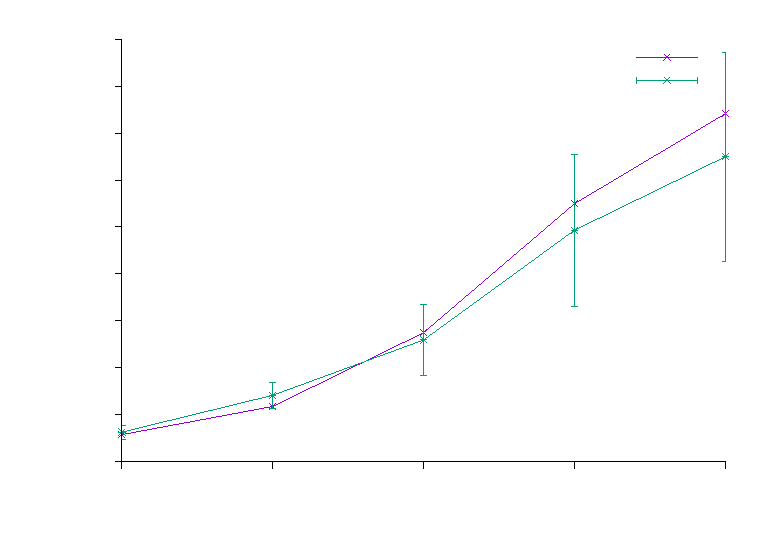
\includegraphics{plot_5}}%
    \gplfronttext
  \end{picture}%
\endgroup
}
  \caption{The flu trend timeline of Dec. 2017}
  \label{figure:5}
\end{figure}


\section{Conclusions}

% 1. Summarize what the major conclusions are
% 2. If your ideas worked, try to provide rationalizations as to why. If not, discuss what may have gone wrong
% 3. In either case discuss what could be done in future to improve or further improve this project
% 1 page

We have developed a twitter-stream text mining and machine learning approach to predict flu outbreaks. 
The proposed method is promising in that it forecasts flu outbreaks in real time. Our method shows a high correlation between the Twitter based prediction
and the groundtruth from CDC report.
The current method heavily relies on the effectiveness of keyword extraction.
The quality of keyword generation depends on the quality of manual labelling as well as the accuracy of the association
between words and the relevant information. It is also worth mentioning that a Twitter stream dataset can be extremely large,
which poses a significant challenge to processing and mining.
In the project we have manually labelled 15,990 tweets and handled 18,938,756 JSON records.

For future work, We can look at employing other natural language processing (NLP) techniques other than simple keyword based analysis, since the context
of a word or sentence is equally important.


\section{Code/Data Release and Individual Tasks}

\subsection{Code/Data Release}

We release our code at \url{https://github.iu.edu/rz20/B565-DataMining}. The Python source code is at the \path{src} directory, where
\path{preprocess} contains the scripts for data preprocessing, \path{labelling} for data labelling and \path{mining} for training
and prediction.

The dataset is stored at \url{https://bit.ly/2r6hle9} (Google Drive IU).

\subsection{Individual Tasks}

We have had regular group meetings every week to synchronize the progress of the project, during which each team member has contributed their thoughts.

\paragraph{Tianyu Chen}
As the team leader, Tianyu worked on preprocessing and dataset handling. He processed the Twitter dataset to suit keyword extraction.
He helped Rui improve the code and Yuhan for manual lablelling. He also performed the experiments of keyword extraction.

\paragraph{Yuhan Zeng}
Yuhan manually labelled more than 10,000 flu-relevant tweet candidates, which is one of the most critical part of this project.
She also worked on keywords extraction and Twitter-based flu trend prediction. She also contributed to the writing of this report.

\paragraph{Rui Zhang}
Rui was responsible for the development of keyword extraction and the neural network predictor. He got preliminary results on the small datasets.
He also performed the experiments on flu trend prediction on the larger datasets and analyzed the results. He wrote the result section of the report.

\bibliographystyle{unsrt}
\bibliography{ref}

\end{document}
